\chapter{Concluding Remarks}
\label{chap:conclusion}

%\epigraph{
%\textit{When information is cheap, attention becomes expensive.}
%}
%{
%--James Gleick, \textit{The Information}
%}
%
%\epigraph{
%\textit{Our task as men is to find the few principles that will calm the infinite anguish
%of free souls. We must mend what has been torn apart, make justice imaginable again in a
%world so obviously unjust, give happiness a meaning once more to peoples poisoned by the
%misery of the century. Naturally, it is a superhuman task. But superhuman is the term
%for tasks men take a long time to accomplish, that's all.}
%}
%{
%--Albert Camus, \textit{The Almond Trees}
%}

\epigraph{
    \textit{The point is there ain't no point.}
}
{
    --Cormac McCarthy, \textit{No Country for Old Men}
}

%\epigraph{
%    \textit{The more the universe seems comprehensible, the more it also seems pointless.
%    But if there is no solace in the fruits of our research, there is at least some consolation
%    in the research itself. Men and women are not content to comfort themselves with tales of
%    gods and giants, or to confine their thoughts to the daily affairs of life; they also build telescopes
%    and satellites and accelerators, and sit at their desks for endless hours working out the meaning of the
%    data they gather. The effort to understand the universe is one of the very few things that lifts
%    human life a little above the level of farce, and gives it some of the grace of tragedy.}
%}
%{
%    --Steven Weinberg, \textit{The First Three Minutes}
%}

\epigraph{
    \textit{The effort to understand the universe is one of the very few things that lifts
    human life a little above the level of farce, and gives it some of the grace of tragedy.}
}
{
    --Steven Weinberg, \textit{The First Three Minutes}
}

%%%%%%%%%%%%%%%%%%%%%%%%%%%%%%%%%%%%%%%%%%%%%%%%%%%%%%%%%%%%%%%%%%%%%%%%%%%%%%%%%%%%%%%%%%%%%%
%%%%%%%%%%%%%%%%%%%%%%%%%%%%%%%%%%%%%%%%%%%%%%%%%%%%%%%%%%%%%%%%%%%%%%%%%%%%%%%%%%%%%%%%%%%%%%
%%%%%%%%%%%%%%%%%%%%%%%%%%%%%%%%%%%%%%%%%%%%%%%%%%%%%%%%%%%%%%%%%%%%%%%%%%%%%%%%%%%%%%%%%%%%%%

\cite{FengNaturalness}

This dissertation has presented work related to the on-going upgrade of the forward muon system
of the ATLAS detector --- the New Small Wheel --- as well as two searches for BSM physics in dilepton final states.
The work thus described has taken place within the years 2015--2019, containing the entirety of the LHC Run 2,
and during a time of change in the physics program of the ATLAS experiment.

At the time of writing in October 2019, the NSW project is on a critical path, at least with respect to its initial timeline of
being fully constructed and installed in ATLAS within the Phase 1 upgrade (c.f. Figure~\ref{fig:lh_schedule}).
In the past few years, the NSW project has seen significant delays.
The construction of large-scale MM and sTGC detectors has never been done prior to the NSW, and
understanding the construction process and behavior of these detectors has been a challenging process
that has, at times, required halting chamber production in order to understand emergent phenomena
that had not been foreseen.
The entire suite of frontend electronics has seen issues, as well, with one of the predominant issues being related to the
design of the ASICs themselves.
The important readout ASIC, the VMM, has had to go through at least one unforeseen design fix to address
issues discovered in the lab, for example.
Even at the time of writing, the current understanding of the yield\footnote{The term `yield' here means
the fraction of produced VMMs that meet the performance criteria for being sufficient for use in ATLAS, and are not
failing specific criteria that are necessary in order to meet the physics goals of ATLAS.}
of the latest version of the VMM ASIC production is unknown.
Understanding this is currently of the utmost priority, since the frontend board development and construction of
detector chambers rely first on their being VMMs on-hand before they themselves can move forward and be fully commissioned.
If this yield is too low, additional ASICs will have to be manufactured at the silicon foundries, which is a lengthy process.
Additionally, the NSW will be the first subsystem of ATLAS to use the upgraded TDAQ system based
on the Front-end Link Exchange (FELIX)~\cite{FELIX} backend.
FELIX, itself, has seen significant delays in its Phase 1 upgrade progress that have led to 
further slowing the progress of the NSW.
With this in mind, the current best foreseen Phase 1 installation plan for the NSW project will be to install only a single wheel
into ATLAS before the start of LHC Run 3, with the second wheel being installed at some point
during Run 3, perhaps during one of the winter shutdown periods.
It may be likely that neither wheels is installed during Phase 1, at which point both wheels will have to be scheduled
for installation in Run 3.
The NSW is a very ambitious project, and such issues as described here are not indicative of those
at the heart of moving it forward but rather a sign of the short window of time that the project
was aiming to be completed in, as well as its having started at a time of great busyness and distraction
at CERN.
% given that the start of the LHC and Higgs discovery happened so near the early days of the NSW project's start.
%had as its goal as well as its having started at a time of great busyness and distraction at CERN, what with the start
%of the LHC and Higgs discovery happening at the time that the NSW as a project was starting.
The current author looks forward to its complete commissioning and smooth operation within the ATLAS experimental cavern,
which will be a testament to the hard work of many, many talented people from around the world having worked together
and designed, built, and butted-heads against a massive project of both new ideas and technologies.


\begin{figure}[!htb]
    \begin{center}
        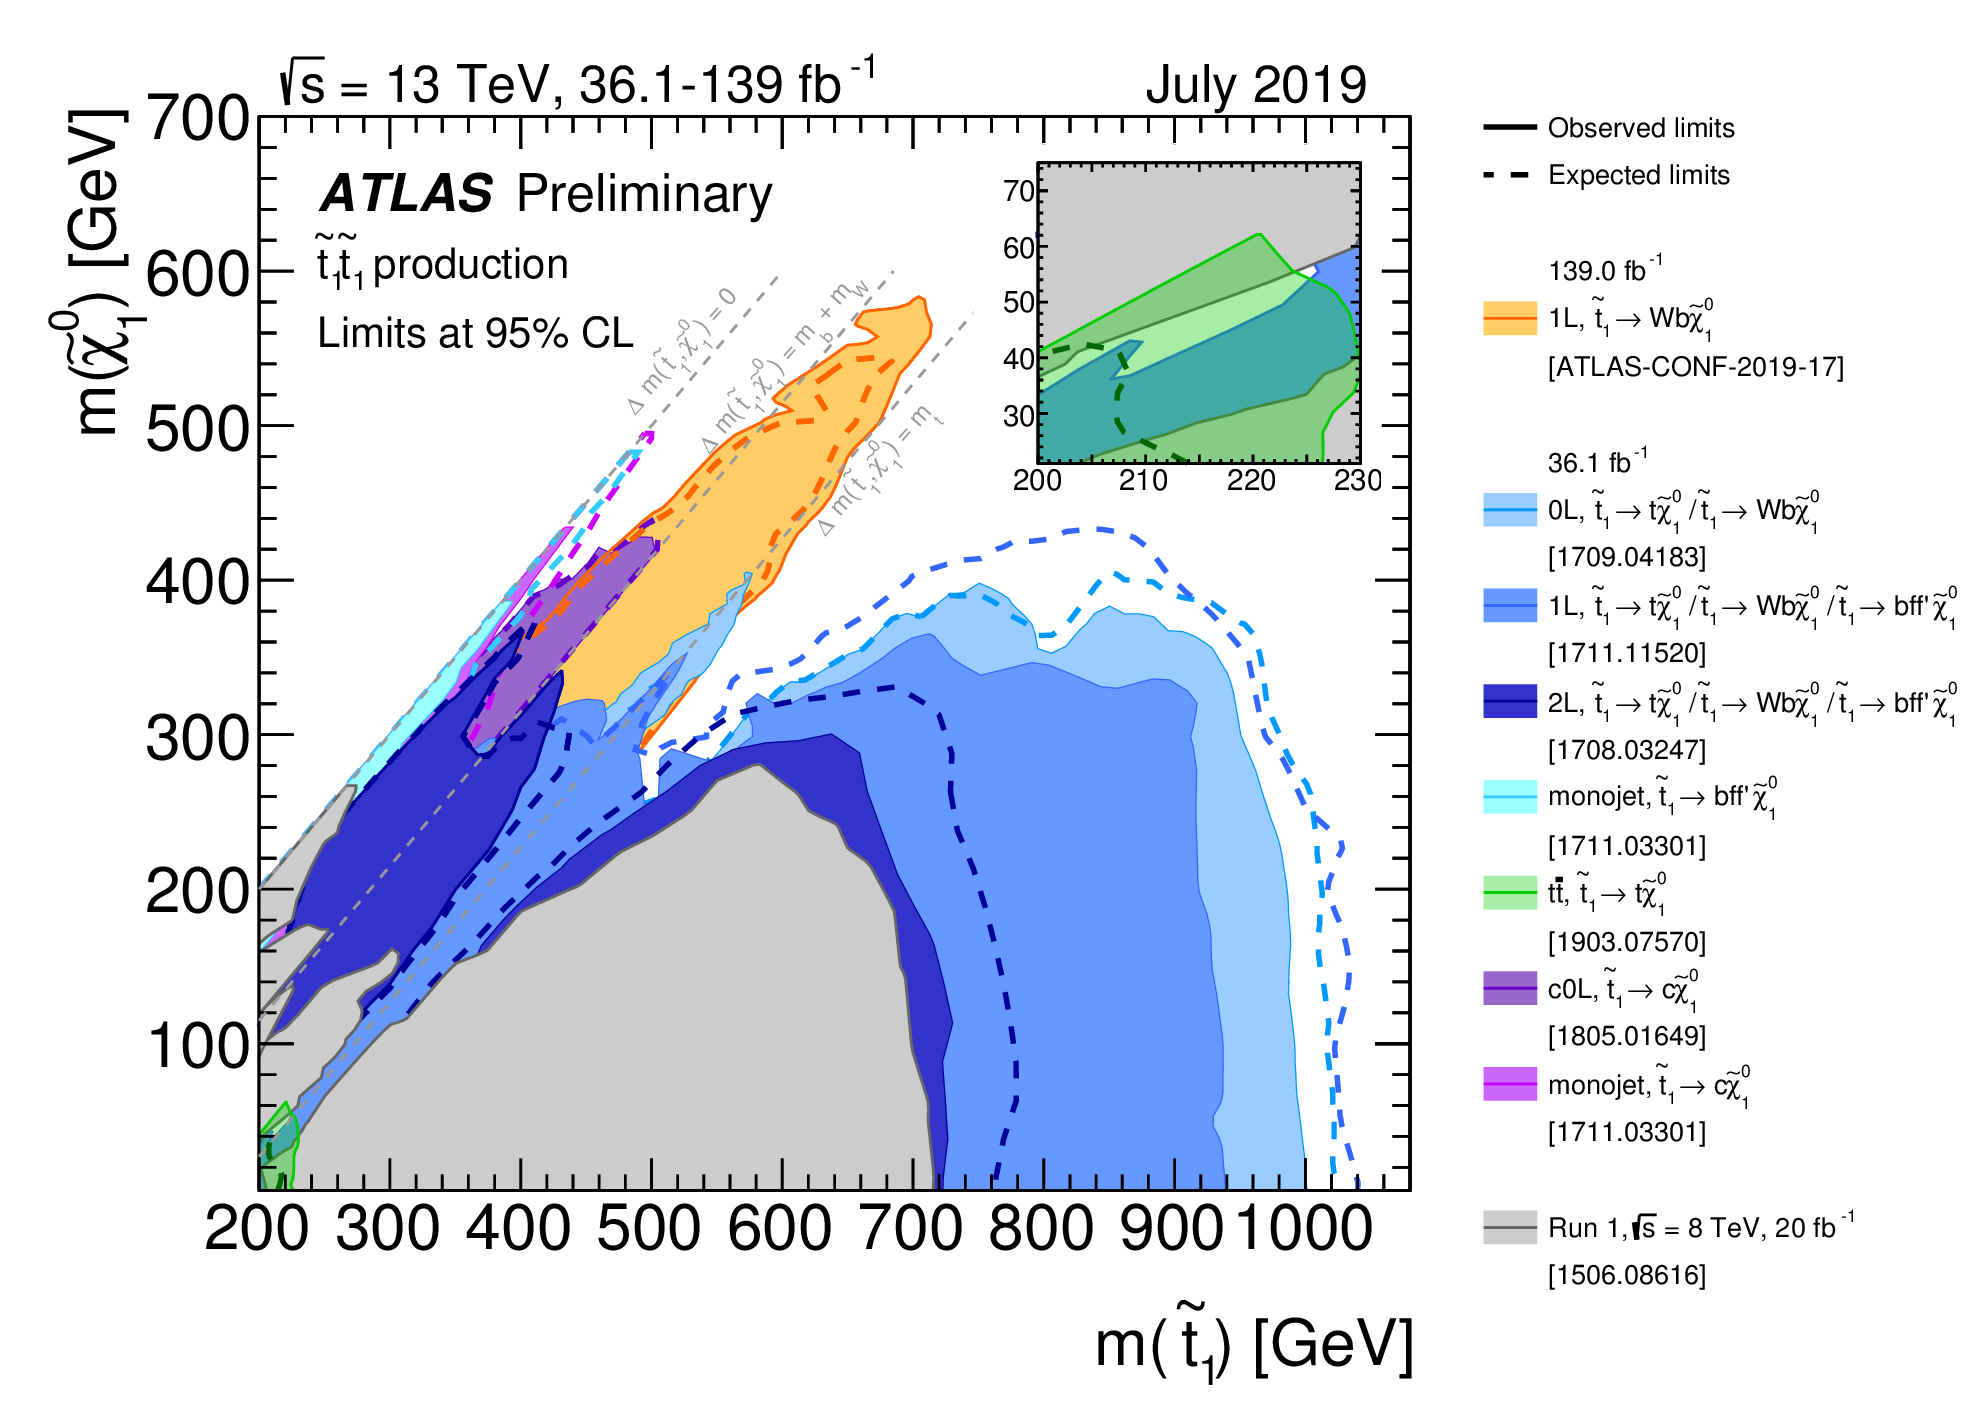
\includegraphics[width=0.85\textwidth]{figures/conclusion/ATLAS_SUSY_Stop_tLSP}
        \caption{
        }
        \label{fig:run2_stop_summary}
    \end{center}
\end{figure}
